\section{Học Liên tục (Continual / Lifelong Learning)}
\label{sec:continual_learning}

\subsection{Động lực: Xây dựng AI Thích ứng với Thế giới Động}
\label{subsec:cl_motivation}
Trong các chương trước, chúng ta đã tập trung vào mô thức huấn luyện "tĩnh" (static) hoặc "ngoại tuyến" (offline): một mô hình được huấn luyện một lần trên một bộ dữ liệu cố định và sau đó được triển khai. Mặc dù phương pháp này đã tạo ra những thành tựu đáng kinh ngạc, nó lại mâu thuẫn với một sự thật cơ bản của thế giới: \textbf{thế giới không ngừng thay đổi}.
\begin{itemize}
	\item Dữ liệu mới xuất hiện liên tục: một hệ thống nhận diện sản phẩm phải học về các mẫu mã mới ra mắt mỗi mùa; một chiếc xe tự hành phải thích ứng với các loại biển báo giao thông hoặc điều kiện đường sá mới ở một quốc gia khác.
	\item Phân phối dữ liệu thay đổi theo thời gian: ánh sáng thay đổi theo mùa, phong cách thời trang thay đổi theo năm.
\end{itemize}
Việc huấn luyện lại toàn bộ một mô hình khổng lồ từ đầu mỗi khi có dữ liệu mới là cực kỳ tốn kém về mặt tính toán, thời gian và tài nguyên. Điều này đặt ra một câu hỏi cơ bản: Làm thế nào để xây dựng các hệ thống AI có khả năng học hỏi và tích lũy kiến thức một cách liên tục, giống như con người, mà không cần phải "học lại từ đầu"?

Câu trả lời nằm ở lĩnh vực \textbf{Học Liên tục (Continual Learning - CL)}, hay còn được biết đến với tên gọi \textbf{Học tập Trọn đời (Lifelong Learning)}. Đây là một mô thức học máy trong đó một mô hình học tuần tự từ một chuỗi các tác vụ (tasks) hoặc các luồng dữ liệu, với mục tiêu học được kiến thức mới trong khi vẫn duy trì được hiệu năng trên các kiến thức đã học.

\subsection{Thách thức Cốt lõi: Quên lãng Thảm khốc (Catastrophic Forgetting)}
\label{subsec:catastrophic_forgetting}
Thách thức lớn nhất và định hình nên toàn bộ lĩnh vực Học Liên tục là hiện tượng \textbf{Quên lãng Thảm khốc (Catastrophic Forgetting)}. Khi một mạng nơ-ron được huấn luyện trên một tác vụ mới (Task B), các trọng số của nó được tối ưu hóa để giảm thiểu hàm mất mát của Task B. Quá trình này thường ghi đè lên các trọng số đã được tối ưu hóa cho tác vụ cũ (Task A), khiến cho hiệu năng của mô hình trên Task A suy giảm nghiêm trọng, thậm chí về mức ngẫu nhiên.

\begin{mdframed}[style=infobox]
	\textbf{Trực giác của Catastrophic Forgetting}
	
	Hãy tưởng tượng một mô hình đã học rất giỏi cách phân biệt giữa "chó" và "mèo" (Task A). Các trọng số trong mạng đã được tinh chỉnh để phát hiện các đặc trưng như tai nhọn, mõm dài, đuôi vẫy,... Bây giờ, chúng ta huấn luyện tiếp mô hình này để phân biệt giữa "ô tô" và "xe đạp" (Task B). Thuật toán tối ưu hóa sẽ điều chỉnh các trọng số để tập trung vào việc phát hiện bánh xe, cửa sổ, tay lái,... Trong quá trình này, các trọng số quan trọng cho việc nhận diện "chó" và "mèo" rất có thể sẽ bị thay đổi hoàn toàn, và mô hình sẽ "quên" mất kiến thức cũ.
\end{mdframed}

Do đó, mục tiêu chính của các thuật toán Học Liên tục là tìm ra cách để học kiến thức mới trong khi vẫn bảo vệ được các kiến thức cũ.

\subsection{Các Chiến lược Chống lại Quên lãng}
\label{subsec:cl_strategies}
Có ba họ chiến lược chính để giải quyết vấn đề Catastrophic Forgetting.

\subsubsection{Các phương pháp dựa trên Chính quy hóa (Regularization-based Methods)}
\label{subsubsec:regularization_based_cl}
Ý tưởng cốt lõi là thêm một thành phần chính quy hóa vào hàm mất mát khi học tác vụ mới. Thành phần này sẽ "phạt" mô hình nếu nó thay đổi các trọng số được cho là quan trọng đối với các tác vụ cũ.
\begin{description}
	\item[Elastic Weight Consolidation (EWC):] \cite{Kirkpatrick2017} Là một phương pháp kinh điển. Sau khi học xong Task A, EWC tính toán "độ quan trọng" của mỗi trọng số $w_i$ đối với Task A. Độ quan trọng này được đo bằng \textbf{Ma trận Thông tin Fisher (Fisher Information Matrix)}. Khi học Task B, hàm mất mát sẽ bao gồm một thành phần phạt, có giá trị lớn nếu các trọng số quan trọng của Task A bị thay đổi nhiều.
	\begin{equation}
		\mathcal{L}_B(\theta) = \mathcal{L}_{\text{Task B}}(\theta) + \frac{\lambda}{2} \sum_i F_i (\theta_i - \theta_{A,i}^*)^2
	\end{equation}
	Trong đó $\theta_{A,i}^*$ là trọng số tối ưu cho Task A, $F_i$ là độ quan trọng (thành phần đường chéo của FIM), và $\lambda$ là hệ số chính quy hóa.
	\item[Learning without Forgetting (LwF):] \cite{Li2017} Thay vì bảo vệ trọng số, LwF bảo vệ output của mô hình. Khi học Task B, ngoài việc học từ nhãn của Task B, mô hình còn được huấn luyện để tái tạo lại các dự đoán (logits) của chính nó trên dữ liệu của Task B \textit{bằng cách sử dụng các trọng số cũ (từ Task A)}. Điều này hoạt động như một hình thức chưng cất tri thức (knowledge distillation) từ "chính mình trong quá khứ".
\end{description}

\subsubsection{Các phương pháp dựa trên Diễn lại (Replay-based Methods)}
\label{subsubsec:replay_based_cl}
Đây là cách tiếp cận trực quan nhất: để không quên, hãy "ôn bài". Các phương pháp này lưu trữ một phần nhỏ dữ liệu từ các tác vụ cũ và trộn chúng vào dữ liệu huấn luyện khi học tác vụ mới.
\begin{itemize}
	\item \textbf{Experience Replay:} Lưu trữ một bộ đệm (buffer) chứa một số lượng nhỏ các mẫu đại diện (exemplars) từ các tác vụ cũ. Phương pháp \textbf{iCaRL} \cite{Rebuffi2017} là một ví dụ điển hình, nó chọn các exemplars là những mẫu gần nhất với trung bình đặc trưng của mỗi lớp.
	\item \textbf{Generative Replay:} Thay vì lưu trữ dữ liệu thực (có thể tốn bộ nhớ hoặc vi phạm quyền riêng tư), phương pháp này huấn luyện một mô hình sinh (như GAN hoặc VAE) trên dữ liệu của Task A. Khi học Task B, nó sử dụng mô hình sinh này để tạo ra các mẫu "giả" của Task A để "ôn lại".
\end{itemize}

\subsubsection{Các phương pháp dựa trên Tách biệt Tham số (Parameter Isolation Methods)}
\label{subsubsec:parameter_isolation_cl}
Ý tưởng của phương pháp này là phân bổ các tài nguyên (tham số) riêng biệt cho mỗi tác vụ để chúng không can thiệp vào nhau.
\begin{itemize}
	\item \textbf{Mở rộng Kiến trúc (Architectural Expansion):} Ví dụ như \textbf{Progressive Neural Networks (PNN)}, mỗi khi có một tác vụ mới, một "cột" (column) mạng mới sẽ được thêm vào. Cột mới này nhận input từ cả dữ liệu đầu vào và các feature map từ các cột cũ, nhưng các cột cũ được "đóng băng" và không bị thay đổi. Cách này hoàn toàn tránh được forgetting nhưng kích thước mô hình tăng lên theo mỗi tác vụ.
	\item \textbf{Học mặt nạ (Mask-based Learning):} Học một "mặt nạ" nhị phân riêng cho mỗi tác vụ, chỉ định các trọng số nào được phép sử dụng và cập nhật cho tác vụ đó.
\end{itemize}

\begin{center}
	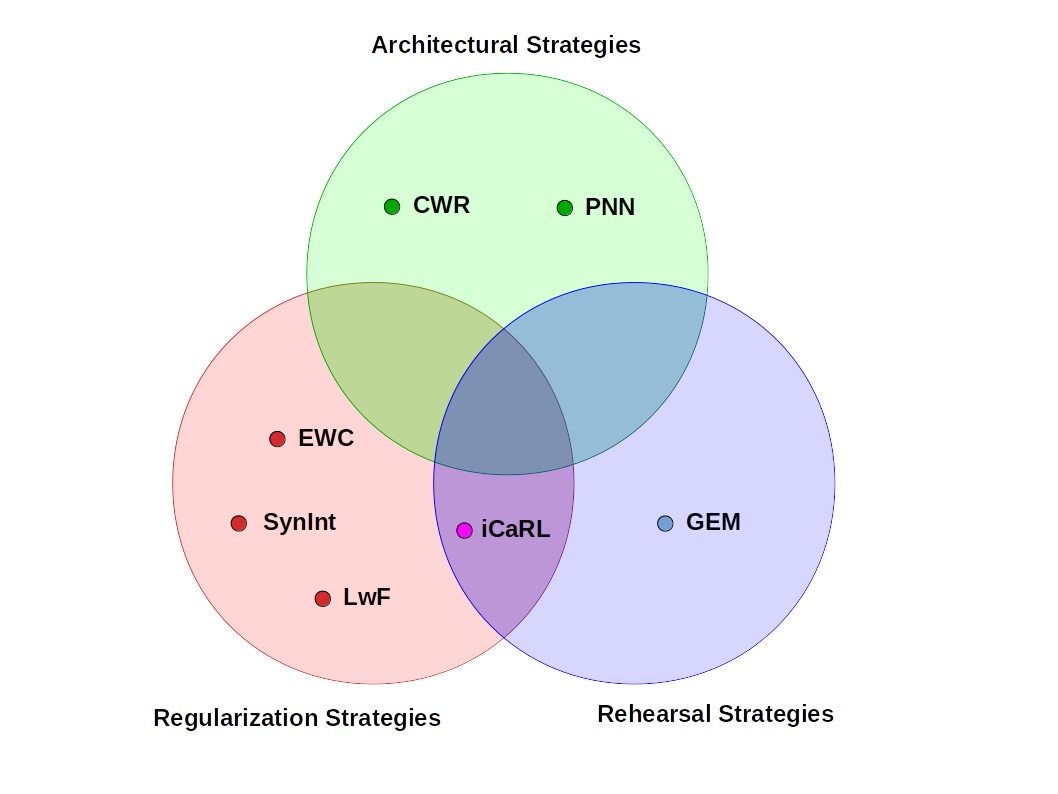
\includegraphics[width=1.0\textwidth]{images/continual_learning_strategies.png}
	\captionof{figure}{So sánh ba chiến lược Học Liên tục chính. (A) Regularization-based: phạt sự thay đổi của các trọng số quan trọng (màu đỏ). (B) Replay-based: lưu trữ các mẫu cũ để ôn lại. (C) Parameter Isolation: cấp phát các tham số riêng cho tác vụ mới.}
	\label{fig:cl_strategies}
\end{center}
% Keyword gợi ý: continual learning strategies, catastrophic forgetting solutions

\subsection{Học Liên tục trong Kỷ nguyên Mô hình Nền tảng}
\label{subsec:cl_foundation_models}
Sự trỗi dậy của các mô hình nền tảng (Foundation Models) được huấn luyện trước trên dữ liệu quy mô lớn đã mở ra một hướng đi mới và cực kỳ hiệu quả cho Học Liên tục.
\begin{itemize}
	\item \textbf{Backbone "Đóng băng":} Các mô hình như CLIP hay DINOv2 đã học được các biểu diễn thị giác cực kỳ tổng quát. Một chiến lược CL hiệu quả là "đóng băng" (freeze) toàn bộ backbone này và chỉ học các thành phần nhỏ, chuyên biệt cho từng tác vụ mới.
	\item \textbf{Prompt-based Continual Learning:} \cite{Wang2022_L2P} Đây là một ví dụ điển hình. Thay vì fine-tune mô hình, chúng ta học một tập hợp các "prompt" (các vector có thể học được, được chèn vào đầu vào của Transformer) riêng cho mỗi tác vụ. Khi gặp một tác vụ, chúng ta chỉ cần tải lên prompt tương ứng. Vì backbone không bị thay đổi, hiện tượng catastrophic forgetting gần như được loại bỏ hoàn toàn. Các phương pháp như \textbf{Learning to Prompt (L2P)} và \textbf{DualPrompt} đã cho thấy hiệu quả vượt trội.
	\item \textbf{Adapter Tuning:} Tương tự như prompting, chúng ta có thể chèn các module "adapter" nhỏ vào giữa các lớp của Transformer và chỉ huấn luyện các adapter này cho mỗi tác vụ mới.
\end{itemize}
Cách tiếp cận này kết hợp sự ổn định của một backbone mạnh mẽ với sự linh hoạt của các thành phần chuyên biệt, nhẹ, tạo ra một giải pháp cực kỳ hiệu quả và tiết kiệm tài nguyên cho Học Liên tục.

\subsection{Kết luận: Hướng tới AI có khả năng Học tập Trọn đời}
\label{subsec:cl_conclusion}
Học Liên tục không còn là một bài toán mang tính lý thuyết. Trong một thế giới nơi dữ liệu không ngừng được tạo ra, khả năng thích ứng và tích lũy kiến thức là một yêu cầu tất yếu đối với các hệ thống AI thông minh. Nó là cầu nối giữa các mô hình "tĩnh" trong phòng thí nghiệm và các tác nhân AI "động" có thể hoạt động bền bỉ trong thế giới thực.

Các chiến lược như regularization, replay, và đặc biệt là các phương pháp dựa trên mô hình nền tảng như prompt tuning, đang dần biến giấc mơ về một AI có khả năng \textbf{học tập trọn đời} thành hiện thực. Một mô hình thực sự thông minh không chỉ là một mô hình mạnh mẽ tại một thời điểm, mà là một mô hình biết cách học hỏi mãi mãi mà không bao giờ quên đi quá khứ. Đây chính là nền tảng cho một thế hệ "AI có khả năng Thích ứng" (Adaptive AI) trong tương lai.

\section*{Tài liệu tham khảo}
\begin{itemize}
	\item[1] Kirkpatrick, J., Pascanu, R., Rabinowitz, N., Veness, J., Desjardins, G., Rusu, A. A., ... \& Hadsell, R. (2017). Overcoming catastrophic forgetting in neural networks. \textit{Proceedings of the national academy of sciences}, 114(13), 3521-3526. (Paper gốc giới thiệu EWC).
	\item[2] Li, Z., \& Hoiem, D. (2017). Learning without forgetting. \textit{IEEE transactions on pattern analysis and machine intelligence}, 40(12), 2935-2947. (Paper gốc giới thiệu LwF).
	\item[3] Rebuffi, S. A., Kolesnikov, A., Sperl, G., \& Lampert, C. H. (2017). icarl: Incremental classifier and representation learning. In \textit{Proceedings of the IEEE conference on computer vision and pattern recognition (CVPR)}. (Paper giới thiệu iCaRL).
	\item[4] Lopez-Paz, D., \& Ranzato, M. (2017). Gradient episodic memory for continual learning. In \textit{Advances in neural information processing systems (NeurIPS)}. (Paper giới thiệu GEM).
	\item[5] Rusu, A. A., Rabinowitz, N. C., Desjardins, G., Soyer, H., Kirkpatrick, J., Kavukcuoglu, K., ... \& Hadsell, R. (2016). Progressive neural networks. \textit{arXiv preprint arXiv:1606.04671}. (Paper giới thiệu PNN).
	\item[6] Wang, Z., Zhang, Z., Lee, C. Y., Zhang, H., Sun, R., Ren, X., ... \& Su, H. (2022). Learning to prompt for continual learning. In \textit{Proceedings of the IEEE/CVF Conference on Computer Vision and Pattern Recognition (CVPR)}. (Paper giới thiệu L2P, một phương pháp prompt-based CL tiêu biểu).
	\item[7] Parisi, G. I., Kemker, R., Part, J. L., Kanan, C., \& Wermter, S. (2019). Continual lifelong learning with neural networks: A review. \textit{Neural Networks}, 113, 54-71. (Một bài tổng quan chi tiết về lĩnh vực Học Liên tục).
\end{itemize}